\section{eo\-State Class Reference}
\label{classeo_state}\index{eoState@{eoState}}
eo\-State can be used to register derivants of {\bf eo\-Persistent}{\rm (p.\,\pageref{classeo_persistent})}.  


{\tt \#include $<$eo\-State.h$>$}

Inheritance diagram for eo\-State::\begin{figure}[H]
\begin{center}
\leavevmode
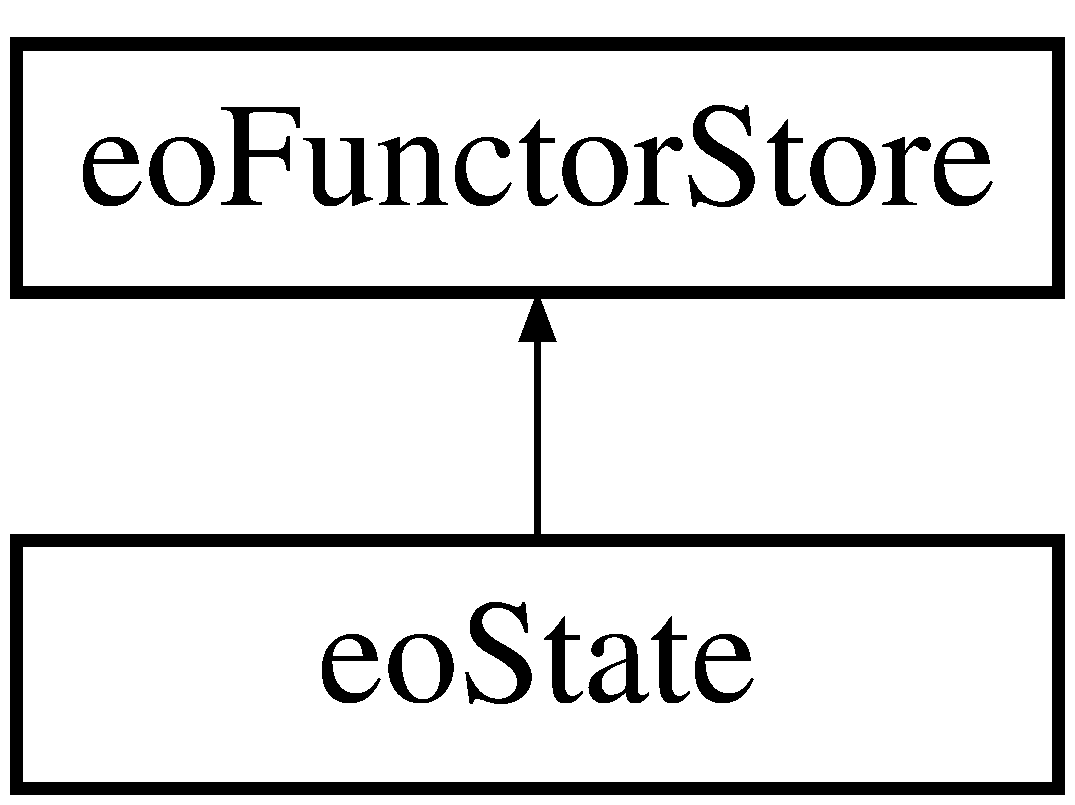
\includegraphics[height=2cm]{classeo_state}
\end{center}
\end{figure}
\subsection*{Public Member Functions}
\begin{CompactItemize}
\item 
void {\bf register\-Object} ({\bf eo\-Persistent} \&registrant)\label{classeo_state_a2}

\begin{CompactList}\small\item\em Object registration function, note that it does not take ownership! \item\end{CompactList}\item 
template$<$class T$>$ T \& {\bf take\-Ownership} (const T \&persistent)
\begin{CompactList}\small\item\em Copies the object (MUST be derived from {\bf eo\-Persistent}{\rm (p.\,\pageref{classeo_persistent})}) and returns a reference to the owned object. \item\end{CompactList}\item 
std::string {\bf get\-Comment\-String} (void) const \label{classeo_state_a4}

\item 
void {\bf load} (const std::string \&\_\-filename)
\begin{CompactList}\small\item\em Reads the file specified. \item\end{CompactList}\item 
void {\bf load} (std::istream \&is)
\begin{CompactList}\small\item\em Reads the file specified. \item\end{CompactList}\item 
void {\bf save} (const std::string \&\_\-filename) const 
\begin{CompactList}\small\item\em Saves the state in file specified. \item\end{CompactList}\item 
void {\bf save} (std::ostream \&os) const 
\begin{CompactList}\small\item\em Saves the state in file specified. \item\end{CompactList}\end{CompactItemize}
\subsection*{Private Types}
\begin{CompactItemize}
\item 
typedef std::map$<$ std::string, {\bf eo\-Persistent} $\ast$ $>$ {\bf Object\-Map}\label{classeo_state_y0}

\end{CompactItemize}
\subsection*{Private Member Functions}
\begin{CompactItemize}
\item 
std::string {\bf create\-Object\-Name} ({\bf eo\-Object} $\ast$obj)\label{classeo_state_d0}

\item 
{\bf eo\-State} (const {\bf eo\-State} \&)\label{classeo_state_d1}

\item 
{\bf eo\-State} \& {\bf operator=} (const {\bf eo\-State} \&)\label{classeo_state_d2}

\end{CompactItemize}
\subsection*{Private Attributes}
\begin{CompactItemize}
\item 
Object\-Map {\bf object\-Map}\label{classeo_state_r0}

\item 
std::vector$<$ Object\-Map::iterator $>$ {\bf creation\-Order}\label{classeo_state_r1}

\item 
std::vector$<$ {\bf eo\-Persistent} $\ast$ $>$ {\bf owned\-Objects}\label{classeo_state_r2}

\end{CompactItemize}


\subsection{Detailed Description}
eo\-State can be used to register derivants of {\bf eo\-Persistent}{\rm (p.\,\pageref{classeo_persistent})}. 

It will then in turn implement the persistence framework through members load and save, that will call read\-From and print\-On for the registrated objects.

It is derived from {\bf eo\-Functor\-Store}{\rm (p.\,\pageref{classeo_functor_store})}, so that it also serves as a place where all those nifty eo functors can be stored. This is useful in the case you want to use one of the make\_\-$\ast$ functions. These functions generally take as their last argument an {\bf eo\-Functor\-Store}{\rm (p.\,\pageref{classeo_functor_store})} (or a state) which is used to hold all dynamically generated data. Note however, that unlike with {\bf eo\-Persistent}{\rm (p.\,\pageref{classeo_persistent})} derived classes, {\bf eo\-Functor\-Base}{\rm (p.\,\pageref{classeo_functor_base})} derived classes are not saved or loaded. To govern the creation of functors, command-line parameters (which can be stored) are needed. 



Definition at line 54 of file eo\-State.h.

\subsection{Member Function Documentation}
\index{eoState@{eo\-State}!takeOwnership@{takeOwnership}}
\index{takeOwnership@{takeOwnership}!eoState@{eo\-State}}
\subsubsection{\setlength{\rightskip}{0pt plus 5cm}template$<$class T$>$ T\& eo\-State::take\-Ownership (const T \& {\em persistent})\hspace{0.3cm}{\tt  [inline]}}\label{classeo_state_a3}


Copies the object (MUST be derived from {\bf eo\-Persistent}{\rm (p.\,\pageref{classeo_persistent})}) and returns a reference to the owned object. 

Note: it does not register the object, this must be done afterwards! 

Definition at line 73 of file eo\-State.h.\index{eoState@{eo\-State}!load@{load}}
\index{load@{load}!eoState@{eo\-State}}
\subsubsection{\setlength{\rightskip}{0pt plus 5cm}void eo\-State::load (const std::string \& {\em \_\-filename})}\label{classeo_state_a5}


Reads the file specified. 

\begin{Desc}
\item[Parameters:]
\begin{description}
\item[{\em \_\-filename}]the name of the file to load from \end{description}
\end{Desc}


Definition at line 74 of file eo\-State.cpp.\index{eoState@{eo\-State}!load@{load}}
\index{load@{load}!eoState@{eo\-State}}
\subsubsection{\setlength{\rightskip}{0pt plus 5cm}void eo\-State::load (std::istream \& {\em is})}\label{classeo_state_a6}


Reads the file specified. 

\begin{Desc}
\item[Parameters:]
\begin{description}
\item[{\em is}]the stream to load from \end{description}
\end{Desc}


Definition at line 87 of file eo\-State.cpp.

References eo\-Persistent::read\-From().\index{eoState@{eo\-State}!save@{save}}
\index{save@{save}!eoState@{eo\-State}}
\subsubsection{\setlength{\rightskip}{0pt plus 5cm}void eo\-State::save (const std::string \& {\em \_\-filename}) const}\label{classeo_state_a7}


Saves the state in file specified. 

\begin{Desc}
\item[Parameters:]
\begin{description}
\item[{\em \_\-filename}]the name of the file to save into \end{description}
\end{Desc}


Definition at line 148 of file eo\-State.cpp.

Referenced by eo\-Timed\-State\-Saver::operator()().\index{eoState@{eo\-State}!save@{save}}
\index{save@{save}!eoState@{eo\-State}}
\subsubsection{\setlength{\rightskip}{0pt plus 5cm}void eo\-State::save (std::ostream \& {\em os}) const}\label{classeo_state_a8}


Saves the state in file specified. 

\begin{Desc}
\item[Parameters:]
\begin{description}
\item[{\em os}]the stream to save into \end{description}
\end{Desc}


Definition at line 161 of file eo\-State.cpp.

References eo\-Printable::print\-On().

The documentation for this class was generated from the following files:\begin{CompactItemize}
\item 
eo\-State.h\item 
eo\-State.cpp\end{CompactItemize}
